\documentclass[12pt]{article}

\usepackage{ctex}
\usepackage{geometry}
\usepackage{enumerate}
\usepackage{amsmath}
\usepackage{float}
\usepackage{subfigure} 
\usepackage{listings}
\usepackage{xcolor}
\usepackage{cases}
\usepackage{amssymb}    %triangleeq
\usepackage{lastpage}   %页码
\usepackage{fancyhdr}   %页眉页脚
\usepackage{graphicx}   %图片引用路径
\usepackage{indentfirst}    %缩进设置
\usepackage{booktabs}
\usepackage{multirow}

\setlength{\parindent}{2em}%缩进设置
\graphicspath{{C:/Users/adm/Desktop/课程文件/科学计算/作业/3.9作业/tex/image}}%图片引用Path,好像并没有什么用

%New colors defined below
\definecolor{codegreen}{rgb}{0,0.6,0}
\definecolor{codegray}{rgb}{0.5,0.5,0.5}
\definecolor{codepurple}{rgb}{0.58,0,0.82}
\definecolor{backcolour}{rgb}{0.95,0.95,0.92}

%Code listing style named "mystyle"
\lstdefinestyle{mystyle}{
  backgroundcolor=\color{backcolour},   commentstyle=\color{codegreen},
  keywordstyle=\color{magenta},
  numberstyle=\tiny\color{codegray},
  stringstyle=\color{codepurple},
  basicstyle=\ttfamily\footnotesize,
  breakatwhitespace=false,         
  breaklines=true,                 
  captionpos=b,                    
  keepspaces=true,                 
  numbers=left,                    
  numbersep=5pt,                  
  showspaces=false,                
  showstringspaces=false,
  showtabs=false,                  
  tabsize=2
}

%"mystyle" code listing set
\lstset{style=mystyle}
\usepackage{indentfirst}
\setlength{\parindent}{2em}%缩进设置

\graphicspath{{images/}}%图片引用Path
\geometry{left=1in,right=0.75in,top=1in,bottom=1in}     %页边距


\lhead{} %左上页眉

\begin{document}
\pagestyle{fancy}
\setcounter{page}{1}
\rhead{Page \thepage\ of \pageref{LastPage}}
%页码设置
\vspace{20pt}
\centerline{{\Large \textbf{计算机模拟 HW1}}}
\vspace{15pt}

\centerline{{\large \textbf{汪奕晨 3180105843}}}
\vspace{15pt}

%============================== Q1 =========================================
%============================= Problem Restatement =============================
\section{Problem Restatement}
Monty Hall Problem为经典的三门问题:

参赛者会看见三扇关闭了的门,其中一扇的后面有一辆汽车,选中后面有车的那扇门可赢得该汽车,另外两扇门后面则各藏有一只山羊。
当参赛者选定了一扇门,但未去开启它的时候,节目主持人开启剩下两扇门的其中一扇,露出其中一只山羊。
主持人其后会问参赛者要不要换另一扇仍然关上的门。问题是:换另一扇门会否增加参赛者赢得汽车的机率。

显然,不换策略的胜率为$\frac{1}{3}$,而简单枚举可以得到换策略的胜率为$\frac{2}{3}$。
为验证这一结果,我们将首先进行 $N$ 次重复测试,然后:
\begin{enumerate}
\item 统计当 $N$ 线性增长时,频率和标准差的变化;
\item 固定 $N$,进行多组实验,统计胜率的随机分布情况,观察其是否呈正态分布。
\end{enumerate}

%=================================== Notations ===========================
\section{Notations}
\begin{table}[H]
  \centering
  \begin{tabular}{cc}
    \hline
    记号 & 含义 \\ \hline
    $N$ &  在一批(batch)中进行单个测试的次数 \\
    $M$ &  进行批测试(batch test)的组数\\ \hline
  \end{tabular}
  \caption{Notations}
  \label{Table Notations}
\end{table}

%============================= Results =============================
\section{Results}
\subsection{实验一:统计当$N$线性增长时,胜率的变化}
让$N$以5为步长,从10线性增长到700。
对每一个$N$进行$batch\_test$,结果如Figure (\ref{fig 1})。
我们可以得到,随着$N$的增加,胜率的逐渐收敛到$\frac{2}{3}$且震荡频率不断收窄

\begin{figure}[H]
  \centering
  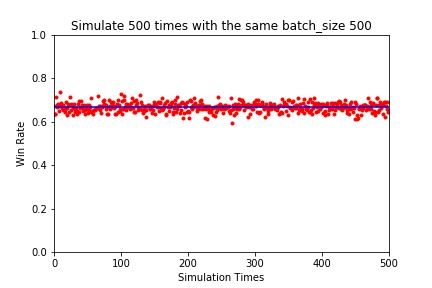
\includegraphics[height = 7cm]{fig3.jpg}
  \caption{The change of win rate as $N$ grows}
  \label{fig 1}
\end{figure}


\subsection{实验二:固定$N$,进行多组实验,统计胜率的分布情况}
固定$N = 500$,进行500次$batch\_test$,得到的胜率分布直方图如Figure (\ref{fig 2}),可以看出胜率大致符合正态分布,我们将在实验三中验证。
\begin{figure}[H]
  \centering
  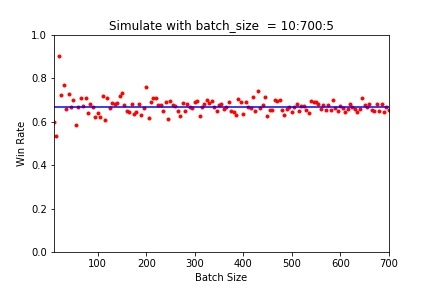
\includegraphics[height = 7cm]{fig2.jpg}
  \caption{The distribution of win rate}
  \label{fig 2}
\end{figure}

\subsection{实验三:检验实验二中的分布是否符合正态分布}
使用Shapiro–Wilk Test检验实验二中的数据,得到的统计量和p值分别为(0.997, 0.450).由统计量接近1且p值显著大于0.05,
可以认为胜率的分布属于正态分布。均值为0.667712,接近我们所期望的$\frac{2}{3}$,可以近似认为该分布属于期望为$\frac{2}{3}$的正态分布。
%============================= Conclution and Disscusion =============================
\section{Conclution and Disscusion}
\subsection{Conclution}
模拟的结果在关于重复次数增长率和大样本(每组 $500$ 次重复,共 $100000$ 组)的结果分布上,均服从期望为 $\frac{2}{3}$ 的正态分布,
从而验证了换门之后,胜率为 $\frac{2}{3}$ 的理论结果。


\subsection{Further Improvement}
\begin{enumerate}
\item 当$N$增长时,估计胜率收敛到$\frac{2}{3}$的速度
\item 根据模拟结果,计算胜率为 $\frac{2}{3}$ 的点估计和区间估计。
\end{enumerate}



%=============================== Appendix =========================================
\section*{Appendix}
\subsection*{Codes}
\begin{lstlisting}[language = Python, caption = ]
  # 引入需要的库
  import pandas as pd  # 用于生成表格
  import numpy as np 
  import matplotlib.pyplot as plt
  from scipy import stats
  
  def init_gates(): # 初始化门的向量
    A = np.zeros(3)  # 三个0标记三个空(无奖)
    n = np.random.randint(3)  # 随机产生一个大奖
    A[n] = 1  # 标记1为大奖
    return A

  def one_sim():  # 进行一次模拟
    G = init_gates() # 三扇门
    award = np.argwhere(G == 1)[0][0]  # 奖所在的门编号 0/1/2
    c = np.random.randint(3) # 随机选择的门
    if c == award:
        a = [0,1,2]
        a.remove(c)
        d = a[np.random.randint(2)] # 主持人删除的门
    else:
        d = 3 - c - award
    # 选择换的策略
    f = 3 - c - d  # 技巧 由于0 1 2 中的两个已知  可以这样得到第三个编号
    if f == award:
        return True
    else:
        return False

  def batch_sim(N): # N为Batch_Size,进行一批模拟
    lst = [one_sim() for i in range(N)]
    win_rate = np.mean(lst)
    return win_rate


  path = './wk1/' # 图片保存路径

  # 多次进行批模拟 改变batch_size
  begin_batch_size = 10  # 起始batch_size
  batch_step = 5 # 步进的batch_size
  end_batch_size = 700 #  最终的batch_size
  
  x = np.arange(begin_batch_size, end_batch_size + batch_step, batch_step)  # batch_size
  y = [batch_sim(i) for i in x]
  
  plt.plot(x,y,'r.')
  plt.plot([begin_batch_size, end_batch_size], [2/3, 2/3], 'b-')
  plt.title('Simulate with batch_size  = {0:d}:{1:d}:{2:d}'.format(begin_batch_size, end_batch_size, batch_step))
  plt.xlabel('Batch Size')
  plt.ylabel('Win Rate')
  plt.axis([begin_batch_size, end_batch_size, 0, 1])
  plt.savefig(path +'fig3.jpg')
  plt.show()

  # 多次进行批模拟的散点图, 不改变batch_size
  batch_size = 500  # 每批重复测试的次数
  sim_size = 500   # 以批为单位模拟的组数
  x = np.arange(sim_size)
  y = [batch_sim(batch_size) for i in x]
  
  plt.plot(x,y,'r.')
  plt.plot([0, sim_size], [2/3, 2/3], 'b-')
  plt.title('Simulate {0:d} times with the same batch_size {1:d}'.format(sim_size, batch_size))
  plt.xlabel('Simulation Times')
  plt.ylabel('Win Rate')
  plt.axis([0, sim_size, 0, 1])
  plt.savefig( path + 'fig1.jpg')
  plt.show()

  plt.hist(y, bins = 32)
  plt.title('Win-rate distribution when N = {0:} and M = {1:}'.format(batch_size, sim_size))
  plt.xlabel('win rate')
  plt.ylabel('counts')
  plt.savefig(path +'fig2.jpg')
  plt.show()

  print(np.mean(y))
  print(np.var(y))
  print(stats.shapiro(y))
\end{lstlisting}
\end{document}